% ══════════════════════════════════════════════════════════════════════════════
%  GMM & EM Section — paste this into the main .tex after the MRF subsection
% ══════════════════════════════════════════════════════════════════════════════

\subsection{Gaussian Mixture Model and EM Algorithm}

While the Bayesian Network and MRF operate on discretized features, we additionally investigate Gaussian Mixture Models (GMMs) fitted via the Expectation-Maximization (EM) algorithm~\cite{dempster1977em} to provide a complementary \textbf{generative, continuous-valued} perspective. EM serves three roles in this project: (1)~principled imputation of missing data, (2)~unsupervised discovery of latent patient phenotypes, and (3)~density-based classification via Bayes' rule. Importantly, EM also underlies parameter learning in BNs with latent variables~\cite{koller2009pgm}, so studying it explicitly on GMMs---where the E- and M-steps have clean closed forms~\cite{bishop2006prml}---provides a foundation for interpreting the algorithm in the more complex graphical model settings discussed above.

\subsubsection{EM for Missing Data Imputation}

The raw dataset contains 6 missing values across \texttt{ca} (4 missing) and \texttt{thal} (2 missing)---the two strongest individual predictors ($r = 0.52$ and $r = 0.51$, respectively). Rather than applying uniform mode imputation, we use the EM algorithm under a multivariate Gaussian assumption $\mathbf{X} \sim \mathcal{N}(\boldsymbol{\mu}, \boldsymbol{\Sigma})$ to compute patient-specific conditional expectations~\cite{little1987rubin}. For each patient $i$ with observed entries $\mathbf{x}_o^{(i)}$ and missing entries $\mathbf{x}_m^{(i)}$, the algorithm iterates:

\begin{itemize}
    \item \textbf{E-step:} Impute missing values via the conditional mean:
    \begin{equation}
        \mathbb{E}[\mathbf{x}_m^{(i)} \mid \mathbf{x}_o^{(i)}, \boldsymbol{\mu}, \boldsymbol{\Sigma}] = \boldsymbol{\mu}_m + \boldsymbol{\Sigma}_{mo}\boldsymbol{\Sigma}_{oo}^{-1}(\mathbf{x}_o^{(i)} - \boldsymbol{\mu}_o)
    \end{equation}
    \item \textbf{M-step:} Re-estimate $\boldsymbol{\mu}$ and $\boldsymbol{\Sigma}$ from the completed dataset.
\end{itemize}

As shown in Figure~\ref{fig:em_imputation}(a), EM imputation converged in just 4 iterations, reflecting the low missingness rate ($\sim$2\%). Unlike mode imputation, which assigns the same value to all patients missing a given feature, EM produces personalized imputations by leveraging each patient's remaining clinical profile. Figures~\ref{fig:em_imputation}(b--c) compare the two strategies: for \texttt{ca}, mode assigns 0 to all four patients, while EM yields values ranging from $-0.25$ to $0.85$ depending on each patient's other measurements.

\begin{figure}[h]
    \centering
    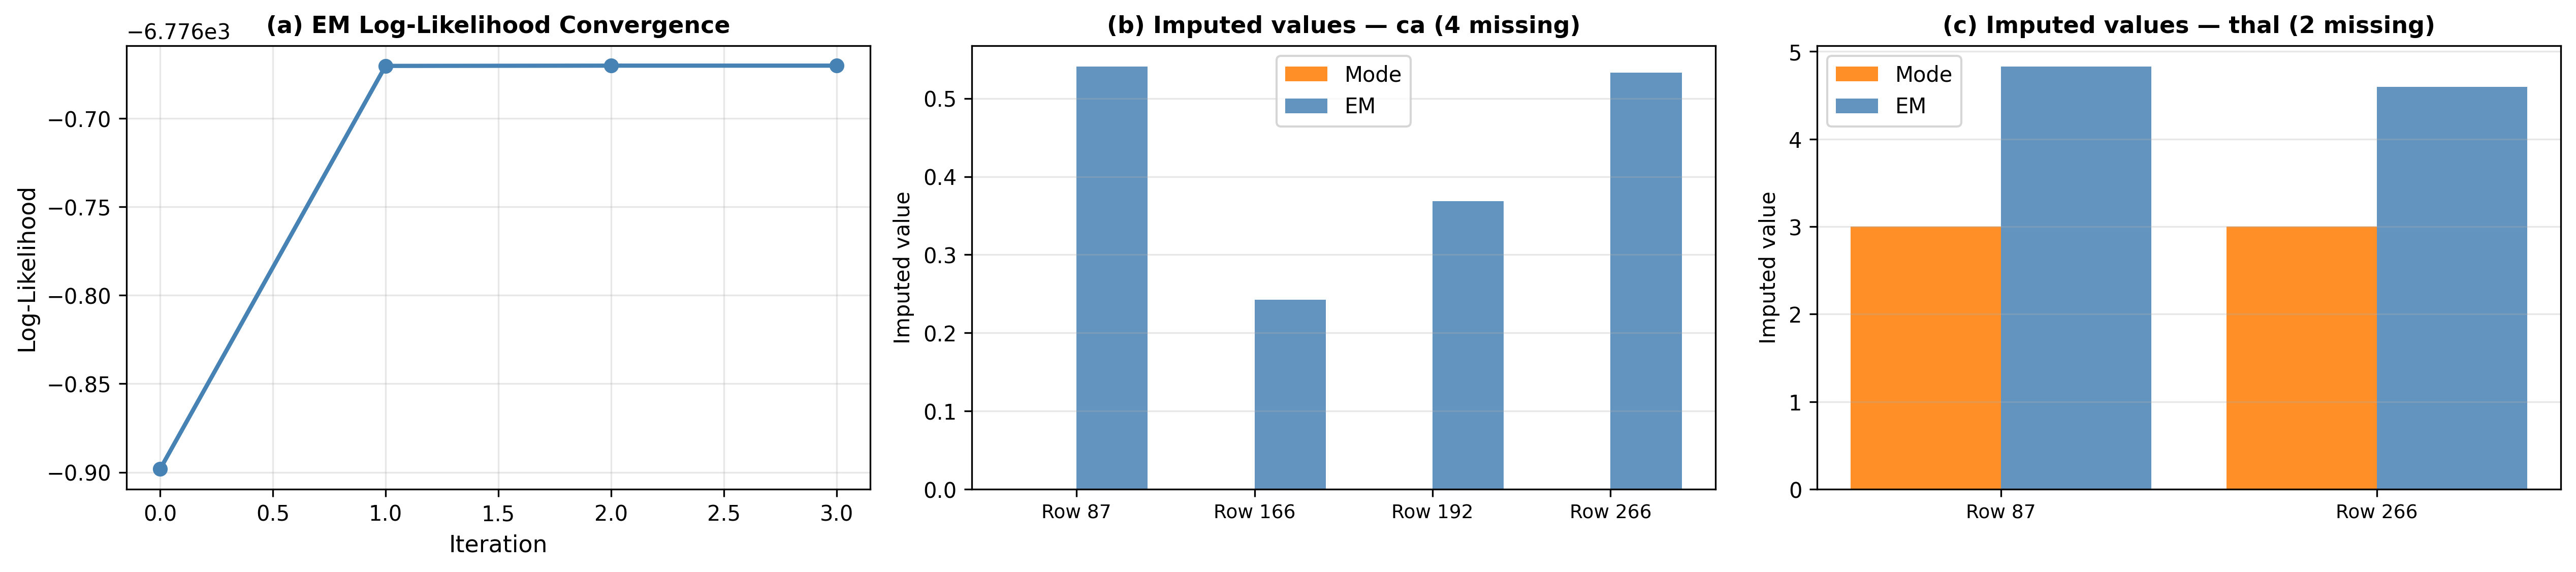
\includegraphics[width=0.95\textwidth]{gmm_em_imputation.png}
    \caption{EM imputation results. (a)~Log-likelihood convergence in 4 iterations. (b--c)~Comparison of mode vs.\ EM imputed values for the 6 missing entries in \texttt{ca} and \texttt{thal}. EM personalizes imputed values based on each patient's observed clinical profile.}
    \label{fig:em_imputation}
\end{figure}

However, a key limitation emerged: the Gaussian assumption produces out-of-range values for inherently discrete features (e.g., \texttt{ca}~$= -0.25$, \texttt{thal}~$\approx 4.6$). This motivates restricting EM imputation to the five purely continuous features (\texttt{age}, \texttt{trestbps}, \texttt{chol}, \texttt{thalach}, \texttt{oldpeak}) for subsequent modeling.

\subsubsection{GMM Clustering and Model Selection}

A Gaussian Mixture Model with $K$ components models the data density as a weighted sum of Gaussians~\cite{mclachlan2000gmm}:
\begin{equation}
    p(\mathbf{x}) = \sum_{k=1}^{K} \pi_k \,\mathcal{N}(\mathbf{x};\,\boldsymbol{\mu}_k,\,\boldsymbol{\Sigma}_k)
\end{equation}
where EM alternates between computing soft responsibilities $r_{ik} \propto \pi_k \,\mathcal{N}(\mathbf{x}_i;\boldsymbol{\mu}_k,\boldsymbol{\Sigma}_k)$ in the E-step and updating $\{\pi_k, \boldsymbol{\mu}_k, \boldsymbol{\Sigma}_k\}$ in the M-step~\cite{bishop2006prml}. We implemented the full algorithm from scratch with log-space computations for numerical stability, and verified correctness against \texttt{sklearn}'s \texttt{GaussianMixture}~\cite{sklearn2011} (Adjusted Rand Index $= 1.0$ for $K\!=\!2$, confirming identical cluster assignments).

To select the number of components, we evaluated BIC~\cite{schwarz1978bic} and AIC for $K = 1, \dots, 8$ on the five standardized continuous features. As shown in Figure~\ref{fig:gmm_bic}(a), BIC selected $K\!=\!2$ as optimal ($\text{BIC} = 3247$), while AIC preferred $K\!=\!5$. BIC's stronger complexity penalty ($p \ln N$) favors parsimony and is more appropriate given the small sample size ($N\!=\!303$), so we adopt $K\!=\!2$.

\begin{figure}[h]
    \centering
    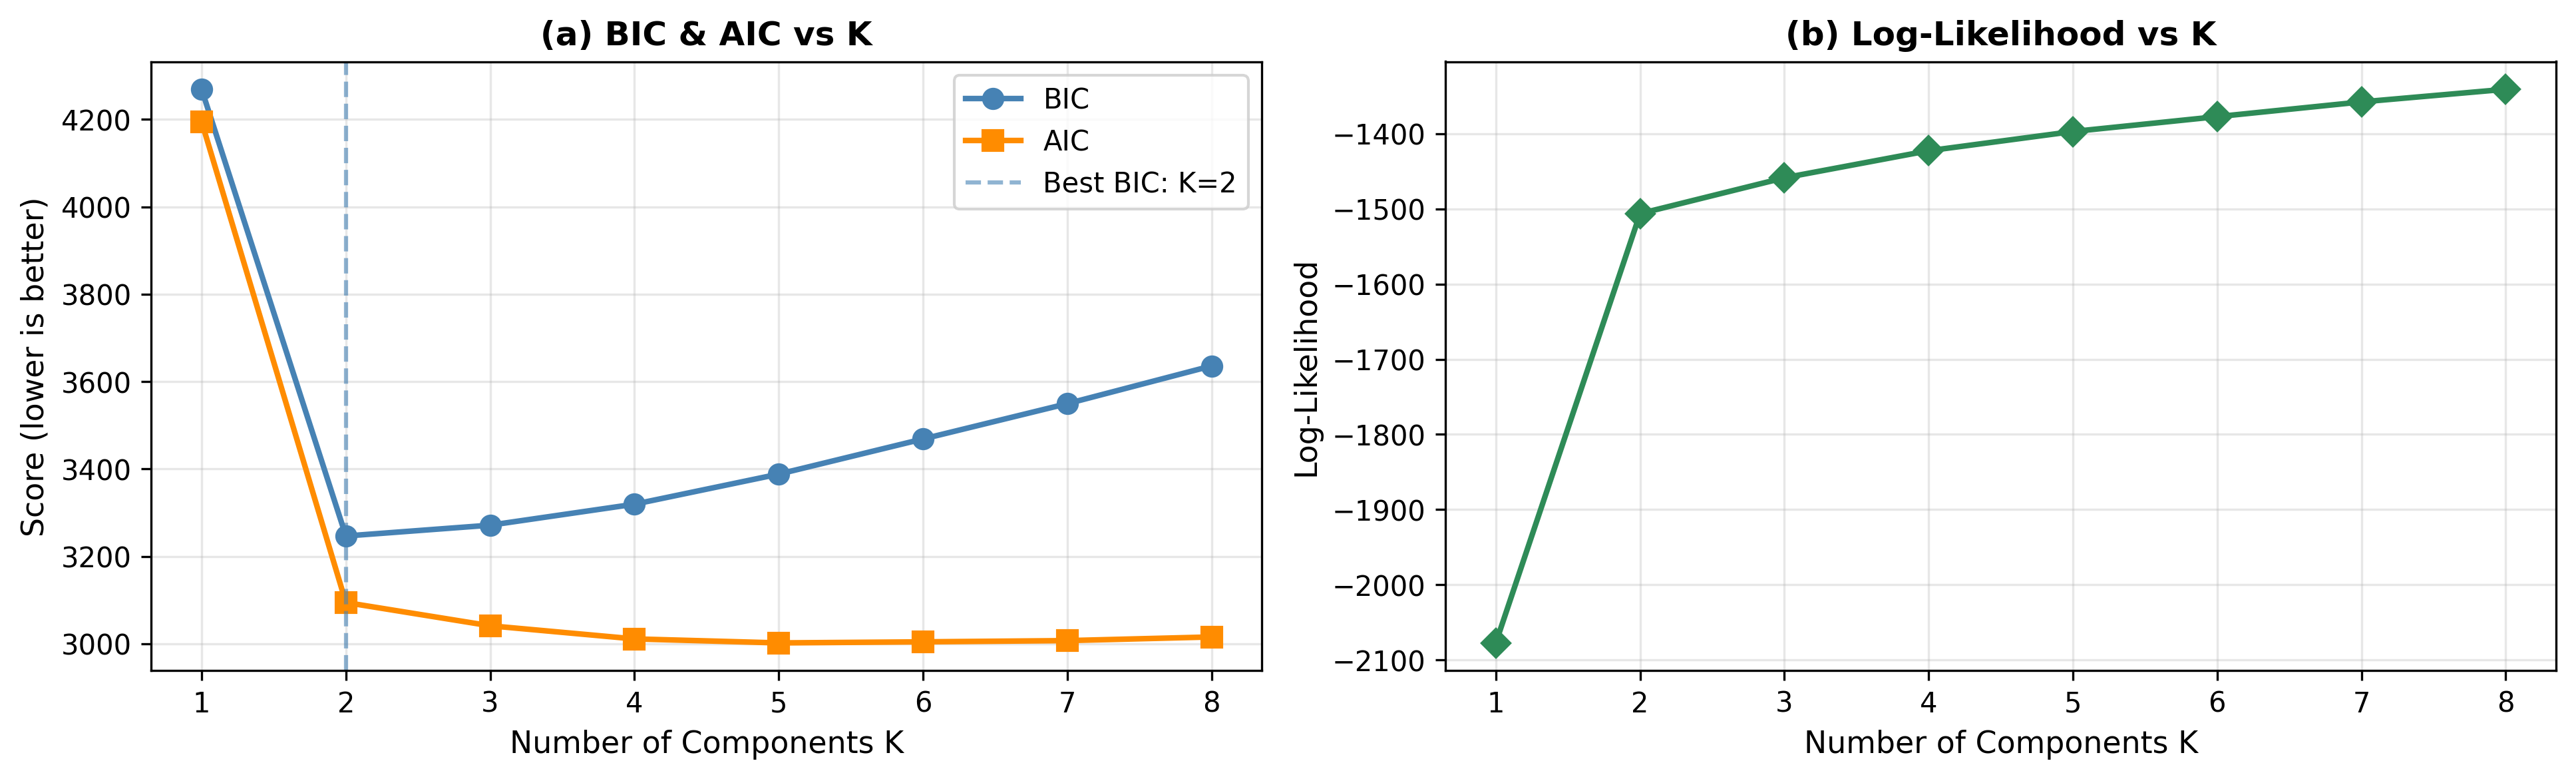
\includegraphics[width=0.95\textwidth]{gmm_bic_aic.png}
    \caption{GMM model selection. (a)~BIC and AIC as a function of $K$; BIC selects $K\!=\!2$. (b)~Log-likelihood increases monotonically, confirming that BIC's parsimony penalty is responsible for the selection of two components.}
    \label{fig:gmm_bic}
\end{figure}

The BIC-optimal two-component solution discovers clinically interpretable patient phenotypes \textbf{without access to the disease label}. Figure~\ref{fig:gmm_clusters}(a) shows the PCA projection of the two GMM clusters alongside the true disease labels in Figure~\ref{fig:gmm_clusters}(b), revealing substantial visual overlap between unsupervised structure and supervised ground truth.

\begin{figure}[h]
    \centering
    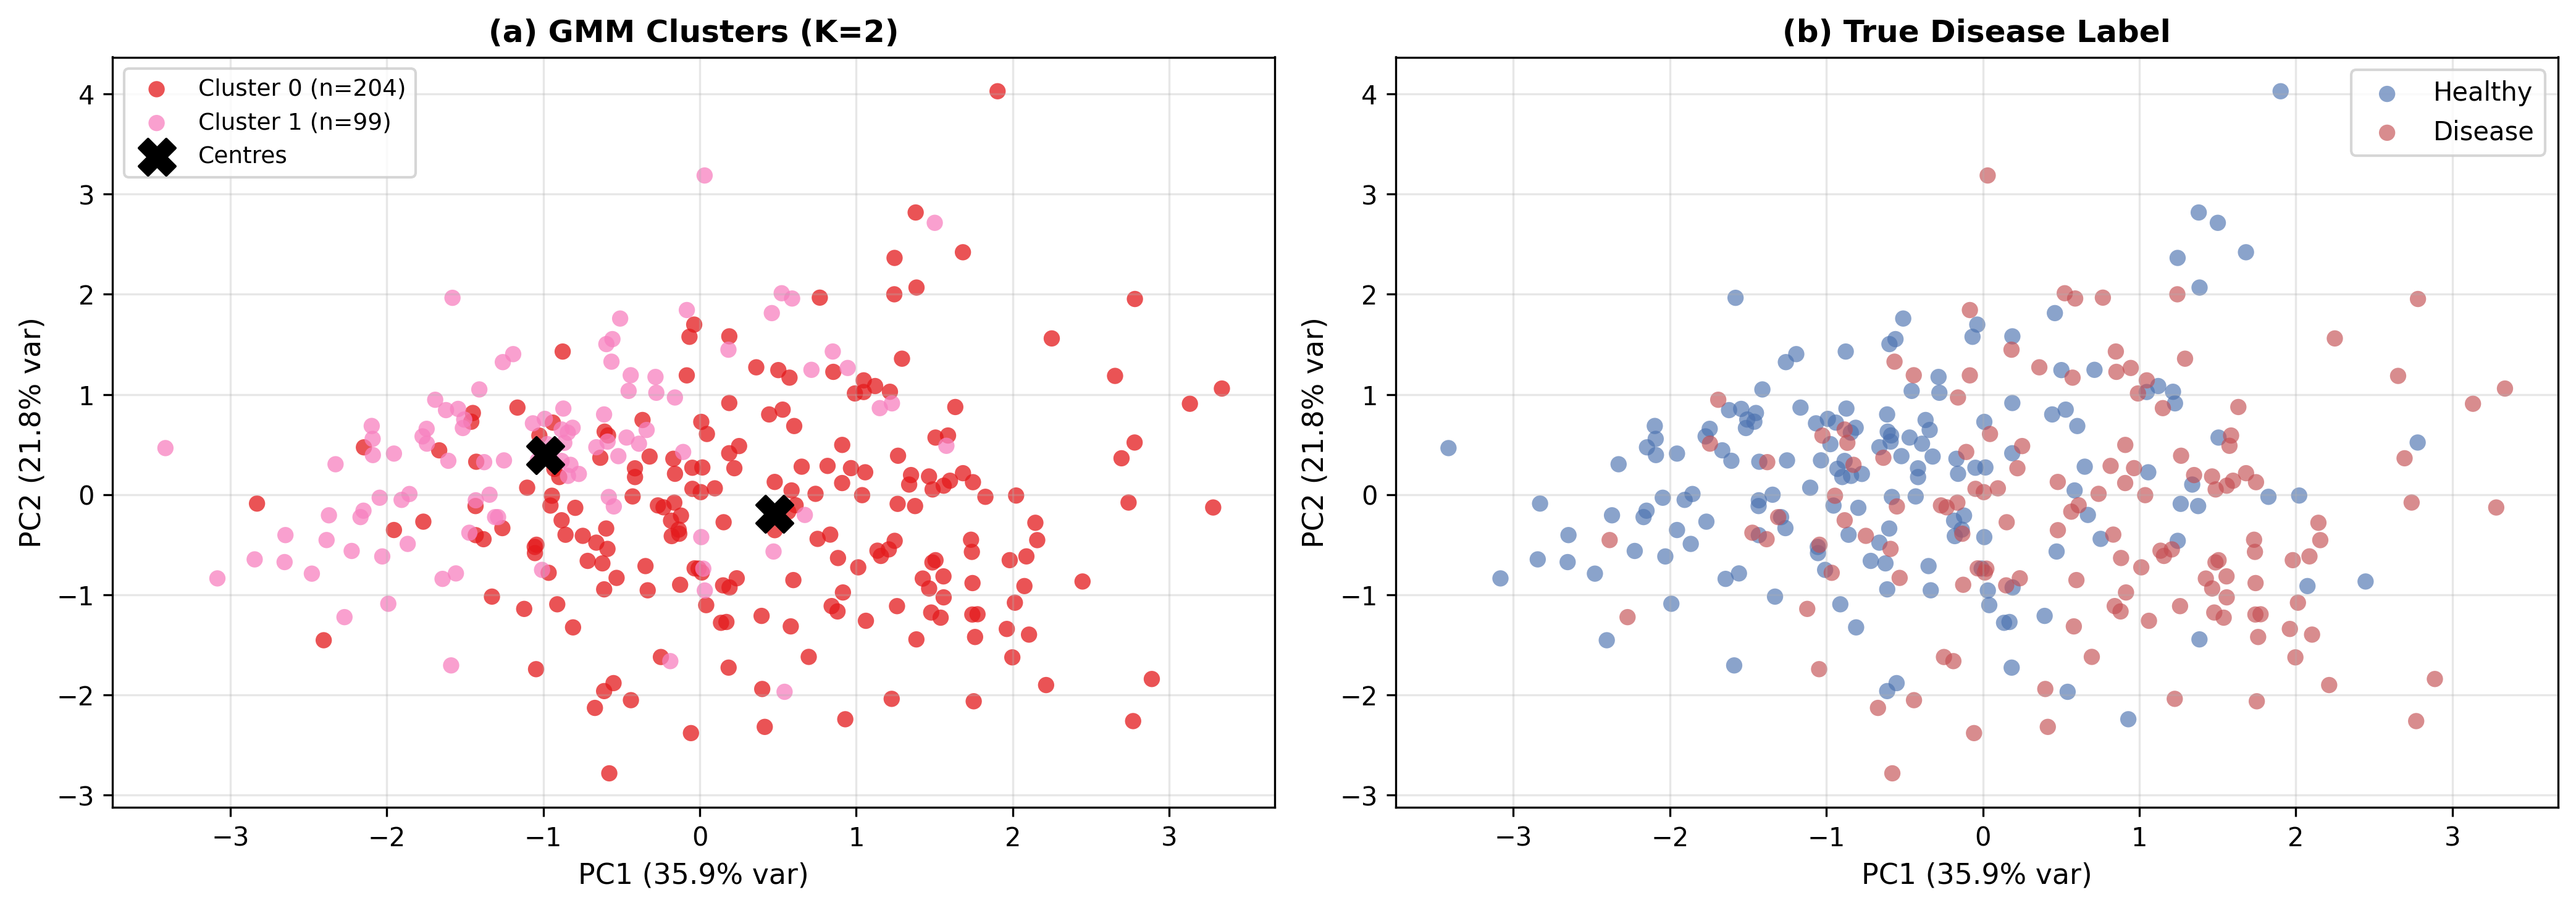
\includegraphics[width=0.95\textwidth]{gmm_pca_clusters.png}
    \caption{PCA projection of the 5-dimensional continuous feature space. (a)~Points colored by GMM cluster assignment ($K\!=\!2$). (b)~Same points colored by true disease label. The unsupervised clusters align substantially with the disease grouping.}
    \label{fig:gmm_clusters}
\end{figure}

Table~\ref{tab:gmm_clusters} summarizes the cluster profiles. Cluster~0 corresponds to a high-risk cardiac profile: older patients with elevated resting blood pressure, significant ST depression under exercise (\texttt{oldpeak}~$= 1.54$), and reduced maximum heart rate---all established markers of compromised myocardial perfusion. Cluster~1 represents younger patients with zero ST depression and higher cardiac reserve. The $2\times$ difference in disease prevalence (55.4\% vs.\ 26.3\%) confirms that the GMM recovers genuine disease-relevant structure from continuous measurements alone.

\begin{table}[h]
\centering
\caption{GMM cluster profiles ($K\!=\!2$, continuous features, original scale). Disease rate is computed from the true labels, which were not used during fitting.}
\label{tab:gmm_clusters}
\begin{tabular}{lrr}
\hline
\textbf{Feature} & \textbf{Cluster 0 (n=204)} & \textbf{Cluster 1 (n=99)} \\ \hline
Age & 56.1 & 51.0 \\
Resting BP (\texttt{trestbps}) & 132.9 & 129.2 \\
Cholesterol (\texttt{chol}) & 248.6 & 242.7 \\
Max Heart Rate (\texttt{thalach}) & 143.6 & 162.1 \\
ST Depression (\texttt{oldpeak}) & 1.54 & 0.00 \\
\textbf{Disease rate} & \textbf{55.4\%} & \textbf{26.3\%} \\ \hline
\end{tabular}
\end{table}

Figure~\ref{fig:gmm_profiles} provides a per-feature breakdown of cluster means. The most striking separation is in \texttt{oldpeak} (1.54 vs.\ 0.00) and \texttt{thalach} (143.6 vs.\ 162.1), consistent with the EDA findings that these exercise-related measurements are among the strongest disease discriminators (Section~3.1).

\begin{figure}[h]
    \centering
    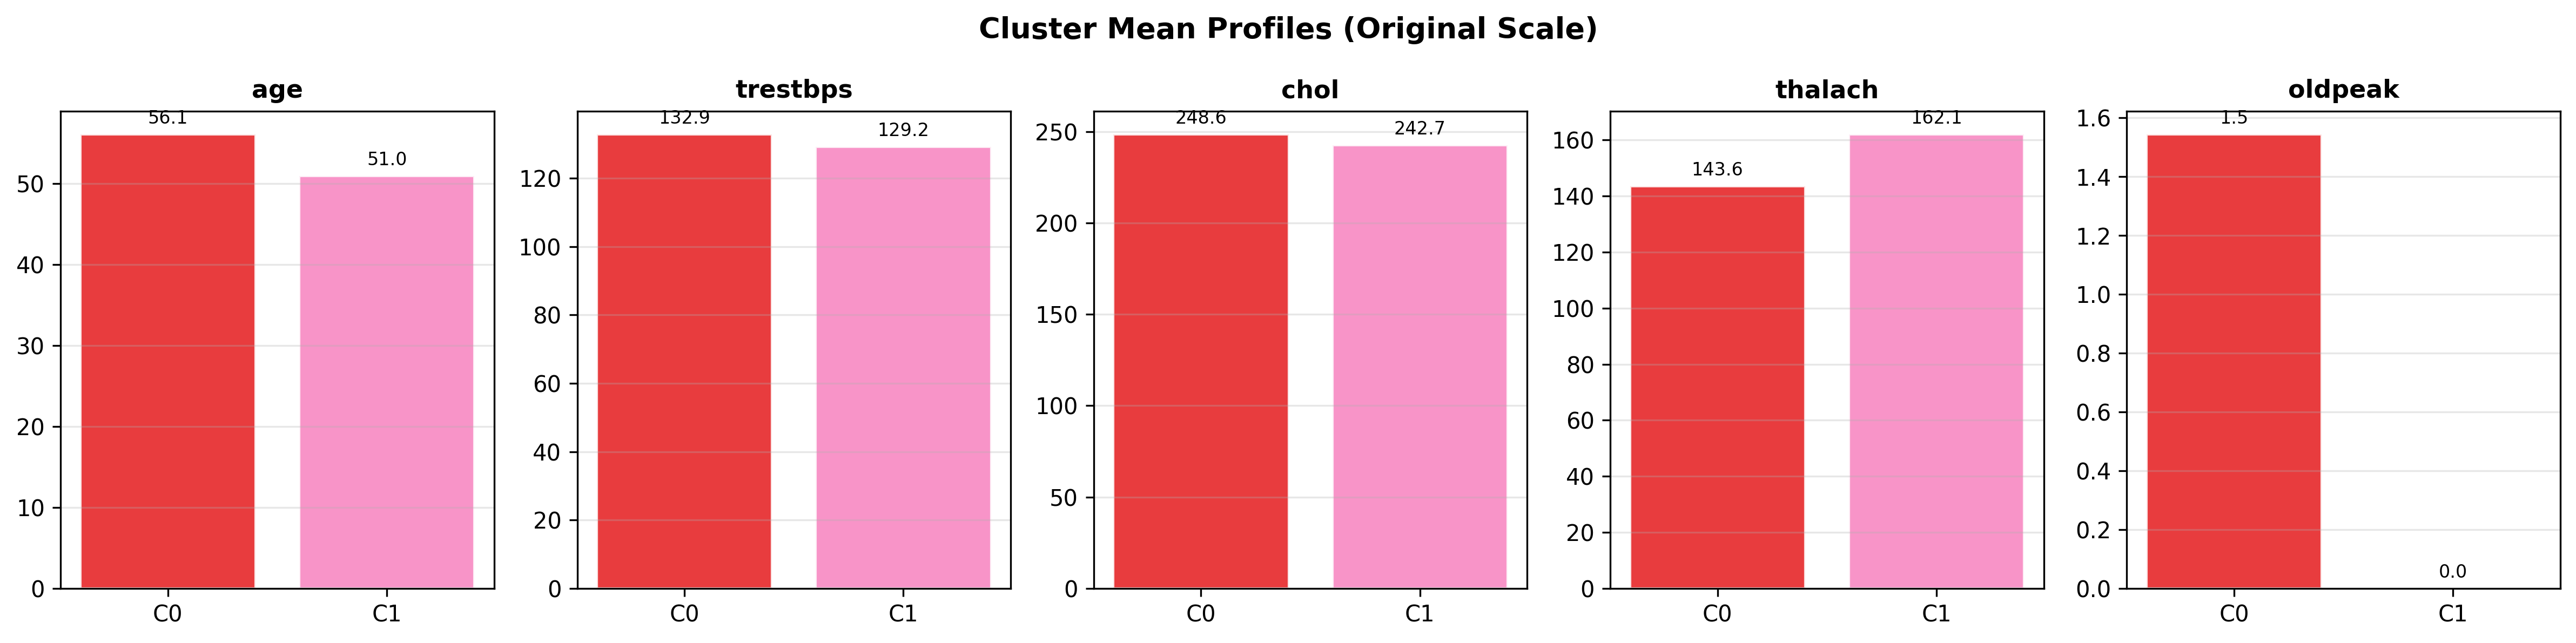
\includegraphics[width=0.95\textwidth]{gmm_cluster_profiles.png}
    \caption{Per-feature cluster mean comparison (original scale). The largest separations appear in \texttt{oldpeak} and \texttt{thalach}, consistent with their strong correlation to disease status.}
    \label{fig:gmm_profiles}
\end{figure}

Notably, soft assignment entropy was near-zero (mean $= 0.003$ bits for both classes), indicating that the two Gaussian components are well-separated in the 5-dimensional feature space. Patients are confidently assigned to one phenotype rather than sitting ambiguously between clusters.

\subsubsection{GMM as a Generative Classifier}

We extend the GMM to supervised classification by fitting a separate class-conditional mixture model and applying Bayes' rule~\cite{murphy2012mlpp}:
\begin{equation}
    P(Y\!=\!1 \mid \mathbf{x}) = \frac{P(\mathbf{x} \mid Y\!=\!1)\,P(Y\!=\!1)}{\sum_{c \in \{0,1\}} P(\mathbf{x} \mid Y\!=\!c)\,P(Y\!=\!c)}
\end{equation}
where each class-conditional density $P(\mathbf{x} \mid Y\!=\!c)$ is a $K\!=\!2$ GMM with full covariance. We evaluate via 5-fold stratified cross-validation on the same five continuous features, comparing against discriminative baselines trained on the identical feature set.

\begin{table}[h]
\centering
\caption{GMM generative classifier vs.\ baselines (5-fold CV, 5 continuous features only). All models use the same restricted feature set for a fair comparison.}
\label{tab:gmm_classifier}
\begin{tabular}{lrrrrr}
\hline
\textbf{Model} & \textbf{Accuracy} & \textbf{F1} & \textbf{AUC} & \textbf{Log Loss} & \textbf{Brier} \\ \hline
GMM Classifier & 0.670 & 0.618 & 0.743 & 0.881 & 0.232 \\
Logistic Regression & \textbf{0.729} & \textbf{0.687} & \textbf{0.794} & \textbf{0.545} & \textbf{0.183} \\
Gaussian NB & 0.720 & 0.674 & 0.793 & 0.626 & 0.195 \\
Random Forest & 0.684 & 0.644 & 0.735 & 0.729 & 0.210 \\
SVM (RBF) & 0.720 & 0.661 & 0.760 & 0.569 & 0.192 \\ \hline
\end{tabular}
\end{table}

As shown in Table~\ref{tab:gmm_classifier} and Figure~\ref{fig:gmm_roc}, the GMM classifier achieves reasonable discrimination ($\text{AUC} = 0.743$) but is consistently outperformed by Logistic Regression and Gaussian Naive Bayes. Three factors explain this gap:

\begin{enumerate}
    \item \textbf{Feature restriction:} Only 5 of 13 features are used because the strongest predictors (\texttt{ca}, \texttt{thal}) are discrete and violate the Gaussian assumption. All models in this comparison therefore operate on a weakened feature set---AUC values here ($\sim$0.74--0.79) are notably lower than the $\sim$0.91 achieved by the same baselines on all 13 features (Table~\ref{tab:bn_comparison}).
    \item \textbf{Small per-class sample size:} With $K\!=\!2$ components per class and $\sim$120 training samples per class per fold, each Gaussian component is estimated from only $\sim$60 observations---insufficient for reliable full-covariance estimation in 5 dimensions.
    \item \textbf{Over-parameterization:} Gaussian Naive Bayes---a special case with $K\!=\!1$ per class and diagonal covariance---outperforms the multi-component GMM ($\text{AUC}$: 0.793 vs.\ 0.743), confirming that the additional mixture components overfit rather than help at this sample size.
\end{enumerate}

\begin{figure}[h]
    \centering
    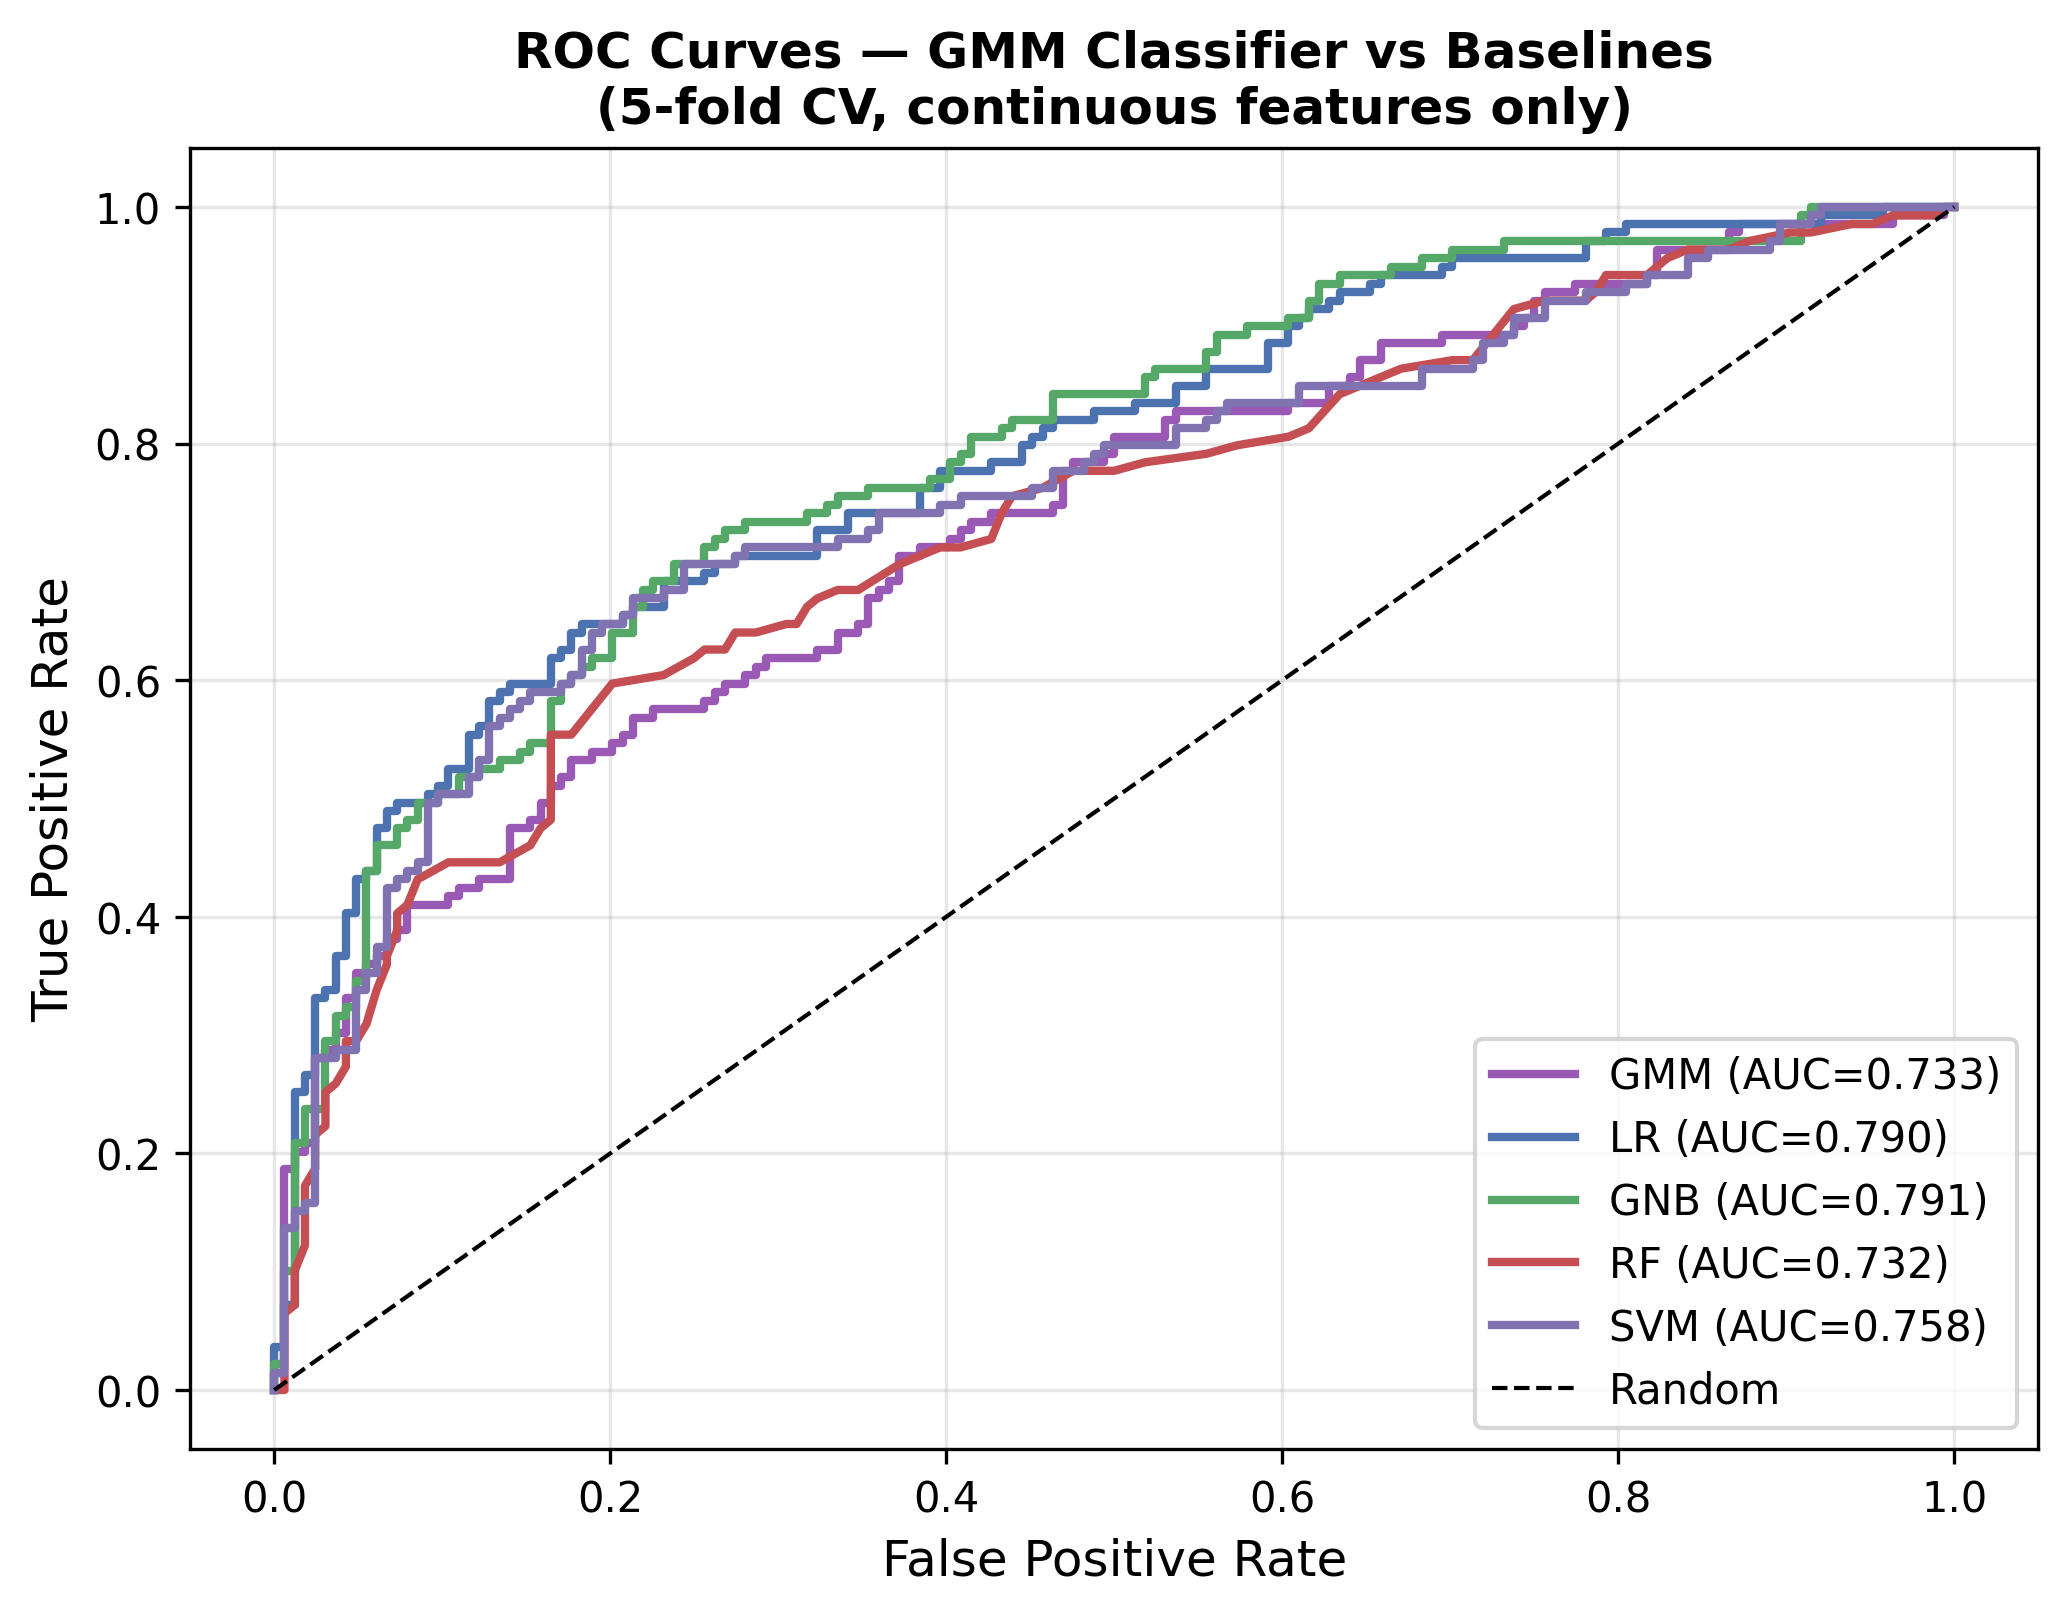
\includegraphics[width=0.65\textwidth]{gmm_roc_curves.png}
    \caption{Pooled ROC curves from 5-fold cross-validation. The GMM classifier achieves reasonable discrimination but is outperformed by Logistic Regression and Gaussian Naive Bayes on the restricted continuous feature set.}
    \label{fig:gmm_roc}
\end{figure}

Figure~\ref{fig:gmm_bars} provides a visual comparison across accuracy, F1, and AUC with error bars indicating cross-fold variability. The GMM classifier exhibits higher variance than Logistic Regression, reflecting sensitivity to fold-level differences in the small dataset.

\begin{figure}[h]
    \centering
    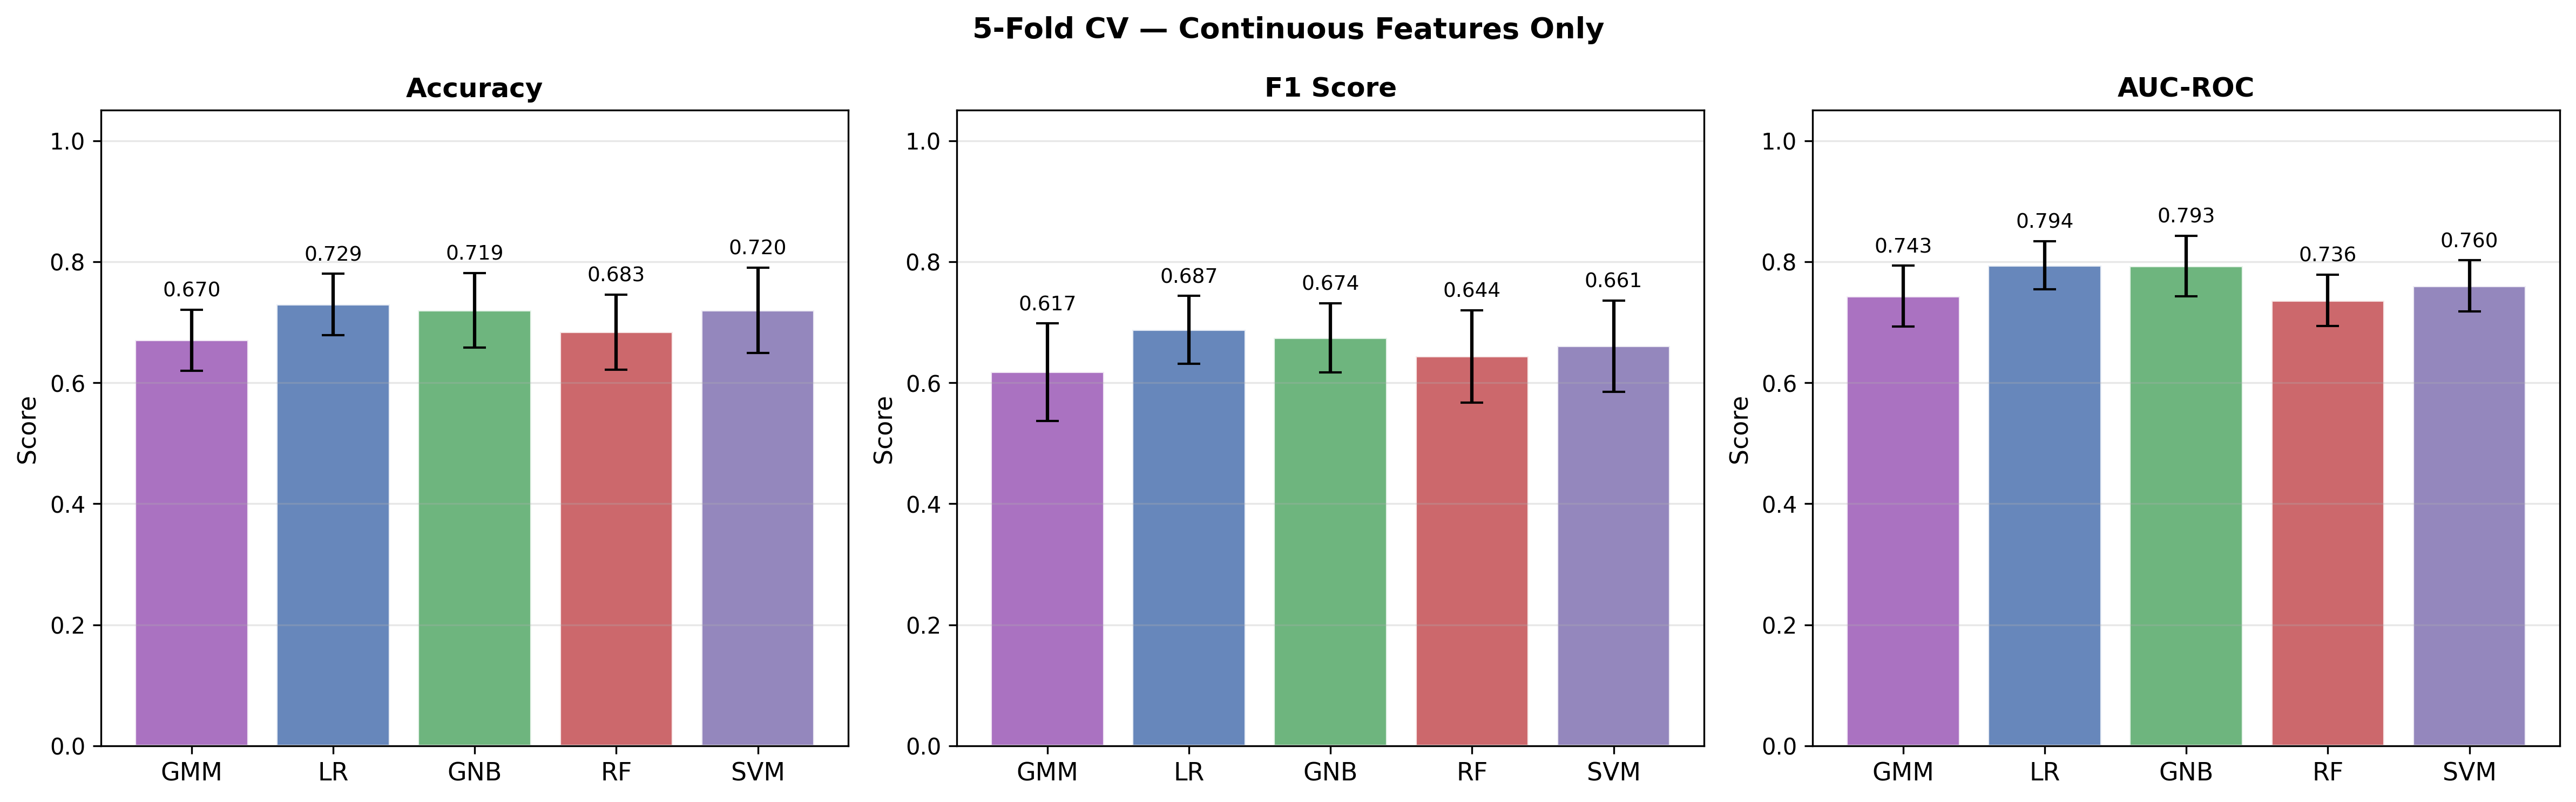
\includegraphics[width=0.95\textwidth]{gmm_performance_bars.png}
    \caption{Performance comparison with standard deviation error bars across 5 folds. All models use 5 continuous features only.}
    \label{fig:gmm_bars}
\end{figure}

\subsubsection{Limitations}

The primary limitation is the Gaussian assumption, which restricts the GMM to continuous features and excludes the two most predictive variables (\texttt{ca} and \texttt{thal}). For EM imputation, this same assumption produces invalid out-of-range values for discrete features; a mixed-type model such as MICE (Multiple Imputation by Chained Equations)~\cite{little1987rubin} would be more appropriate for datasets with both continuous and categorical variables. Additionally, the small sample size penalizes the multi-component GMM classifier relative to simpler parametric models. Despite these limitations, the GMM's primary contribution lies in unsupervised phenotyping and density estimation---providing a generative complement to the discriminative and graphical models evaluated elsewhere in this study.
